\chapter{Architektur\label{chap3:Drittes-Kapitel}}

Für die Architektur der mobilen Anwendung \glqq Geogram\grqq{}, wurden die zwei Frameworks \glqq Ionic\grqq{} und \glqq Express\grqq{} und die Entwicklungs-Plattform \glqq Firebase\grqq{} verwendet.

Wie in \autoref{fig:technologie} veranschaulicht, wird das Web-Framework \glqq Ionic\grqq{} für das Frontend verwendet. Das Backend kann in zwei Bereiche unterteilt werden. Zum einen wird die Entwicklungs-Plattform \glqq Firebase\grqq{} und das Node.js Web-Framework \glqq Express\grqq{} verwendet. Genauere Informationen bezüglich der Aufteilung des Backends wird in \autoref{sec3.2:Unterpunkt-2} beschrieben.

\begin{figure}[H]
    \centering
    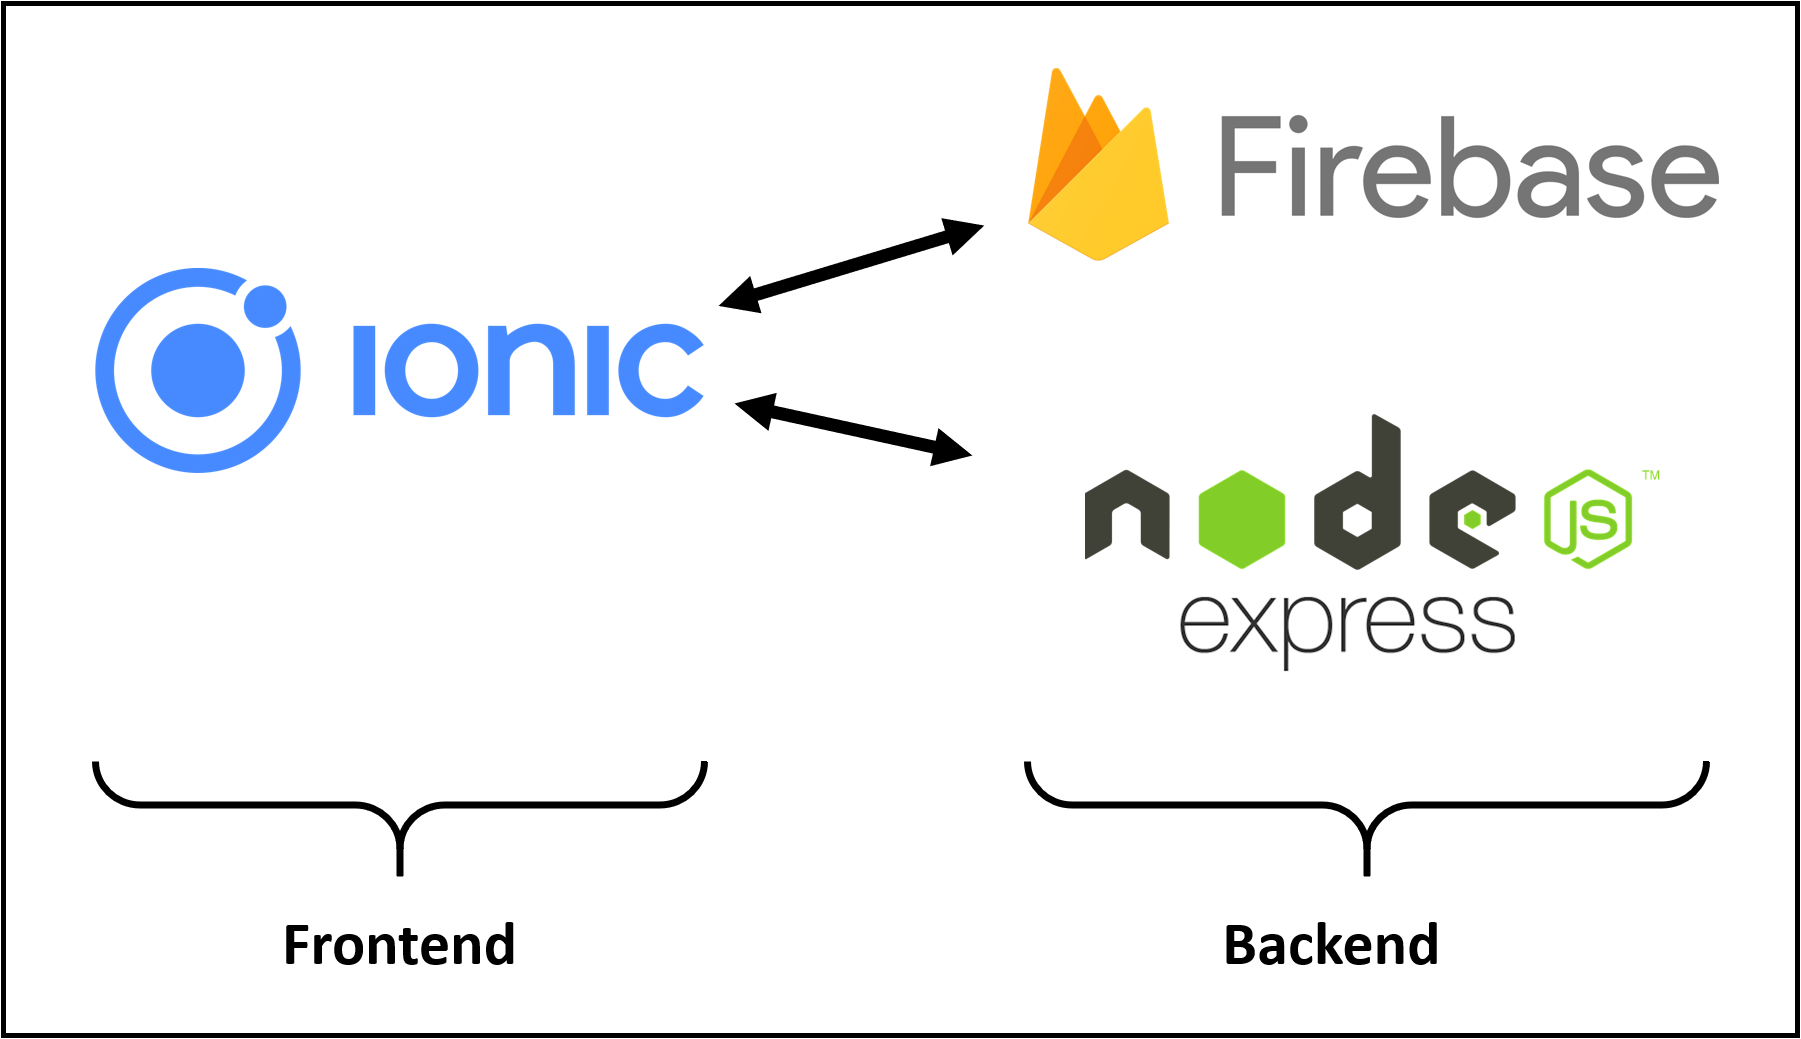
\includegraphics[width=.8\linewidth]{images/Architektur.png}
    \caption{Technologieübersicht}
    \label{fig:technologie}
\end{figure}

\section{Frontend\label{sec3.1:Unterpunkt-1}}

Für die Umsetzung des Frontend wurde das Framework \glqq Ionic\grqq{} verwendet.

Ein Vorteil von Ionic ist es, dass der Code nicht für jede Platform einzeln geschrieben werden muss. Als Entwickler ist man dadurch nicht verpflichtet nativen Code zu implementieren.

Jene Platform unabhängige Entwicklung ist durch den Einsatz von \glqq Ionic Tags\grqq{} möglich. Diese speziellen HTML-Elemente gewährleisten, dass das \glqq Look and Feel\grqq{} der App auf allen Platformen gegeben ist.

In \autoref{fig:ionicModules} sind die in der App \glqq Geogram\grqq{} verwendeten Ionic Tags abgebildet.

\begin{figure}[H]
    \centering
    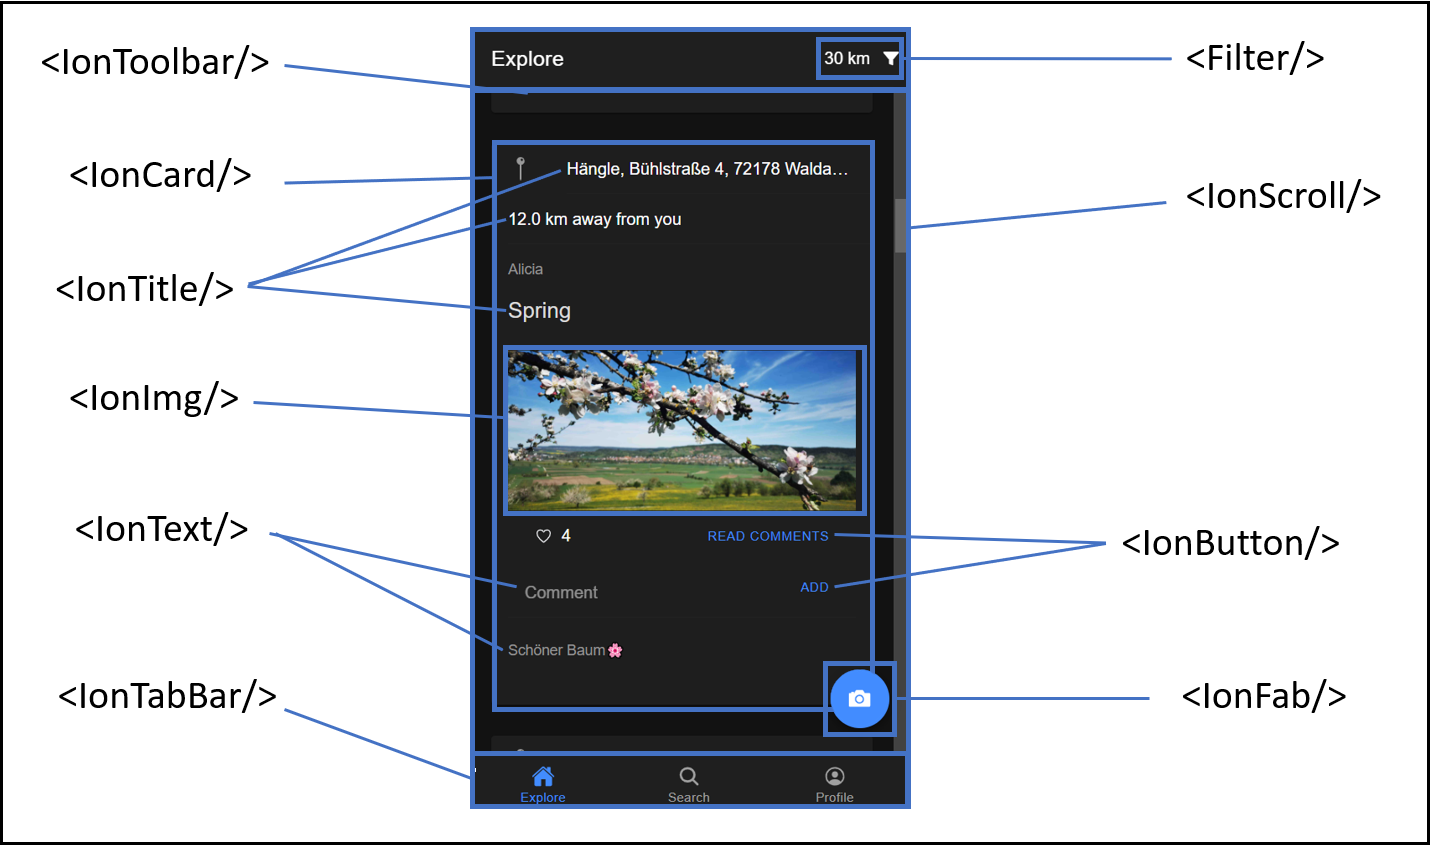
\includegraphics[width=.8\linewidth]{images/ionicModules.png}
    \caption{Ionic Tags}
    \label{fig:ionicModules}
\end{figure}

Damit die Bilder beim Hochladen auch geografische Informationen besitzen, wird mittels Ionic auf die GPS-Sensoren der Geräte zugegriffen. In \autoref{lst:codeGeolocation} ist genau jene Abfrage zu finden. Um die erhaltenen Längen- und Breitengrade in bekannte Straßen und Städte umzuwandeln, wird in Zeile 19 auf eine externe Dienstleistung zurückgegriffen.

\begin{lstlisting}[label=lst:codeGeolocation, caption={Implementierung der GPS-Abfrage}, captionpos=b, breaklines=true]
...
// get current geolocation
Geolocation.getCurrentPosition().then((location) => {
    setLocation({
    coords: {
        accuracy: location.coords.accuracy,
        altitude: location.coords.altitude,
        altitudeAccuracy: location.coords.altitudeAccuracy,
        heading: location.coords.heading,
        latitude: location.coords.latitude,
        longitude: location.coords.longitude,
        speed: location.coords.speed,
    },
    timestamp: location.timestamp,
    });
    // reverse geolocation
    axios
    .get(
        `https://api.opencagedata.com/geocode/v1/json?q=${location?.coords.
        latitude}+${location?.coords.longitude}&key=bb44e70b618844faba7c
        b23b580419e0`
    )
    .then((res) => {
        setPosition(res.data.results[0].formatted);
        setLocation((state: any) => {
        return {
            ...state,
            position: res.data.results[0].formatted,
        };
        });
    });
});
...
\end{lstlisting}

\section{Backend\label{sec3.2:Unterpunkt-2}}

Den Großteil der Backend-Aufgaben übernimmt die Entwicklungsplatform Firebase. Verwendet wird hierfür die kostenlose \glqq Spark Plan\grqq{}-Version von Firebase. 

Die \textbf{Authentifizierung} und das \textbf{Credentialmanagent} wird hierbei vollständig von Firebase übernommen und verwaltet. Über vordefinierte Programmierschnittstellen kann man anschließend auf die Funktionen von Firebase zugreifen. Ebenso wird im kostenlosen Lizenzmodell \glqq Spark Plan\grqq{} eine Cloud-Speicherung namens \glqq \textbf{Firestore}\grqq{} angeboten. In der darin enthaltenen \textbf{Echtzeitdatenbank} stehen jedoch nur 1 GiB Speicherplatz zur Verfügung. Da sich das Kernkonzept von Geogram hauptsächlich um Fotos dreht und die finanziellen Mittel der Gruppe nicht für ein kostenpflichtiges Lizenzmodell ausreichen, wurde zusätzlich ein \textbf{Foto-Server} mithilfe des Web-Frameworks \glqq Express\grqq{} implementiert. Der Foto-Server wird von der Projekt-Gruppe selbst gehostet und beinhaltet mehr als 1 Gib Speicherplatz.

\subsection{Credentialmanagent\label{sup3.2.1:Unterpunkt-1}}

Die Verwaltung von Anmeldeinformationen wird in Geogram von der Entwicklungs-Plattform Firebase übernommen. Firebase bietet verschiedene Sign-in Methoden an. Neben der klassischen E-Mail/Passwort Kombination stellt Firebase noch die Sign-in Methoden von anderen Anbietern zur Verfügung. So kann man die Benutzerkonten von zum Beispiel Google, Facebook, Twitter oder GitHub für die Verwendung verwenden.

Für die mobile Anwendung Geogram wird die klassische Sign-in Methode \glqq E-Mail und Passwort\grqq{} und die Sign-In Methode \glqq Google\grqq{} verwendet.

\subsection{Cloud Firestore\label{sup3.2.2:Unterpunkt-2}}

Die verwendete Firestore-Datenbank ist eine in der Cloud gehostete NoSQL-Datenbank. Über native SDKs können die iOS-, Android- und Web-Apps auf Firestore zugreifen.

\begin{wrapfigure}{r}{0.3\textwidth}
    \begin{center}
        
\includegraphics[width=0.3\textwidth]{images/firestore.png}
    \end{center}
    \caption{Speicherstruktur Firestore}
    \label{fig:storagestructure}
\end{wrapfigure}

In dem NoSQL-Datenmodell von Firestore, werden die Daten in Dokumente gespeichert, welche Felder enthalten, denen Werte zugeordnet sind. Diese Dokumente wiederrum werden in Sammlungen (collections) abgespeichert. Diese hierarchische Rangordnung der Datenspeicherung ist nochmals in \autoref{fig:storagestructure} abgebildet.

Für Geogram werden die zwei Sammlungen \glqq images\grqq{} und \glqq users\grqq{} benötigt. Wie die Bezeichnungen schon vermuten lassen, werden darin die Fotos und die Benutzer von Geogram abgespeichert.

Die Dokumente der Sammlung \glqq users\grqq{} bilden die verschiedenen Benutzerprofile von Geogram ab. Ein Benutzerprofil wird durch folgende Felder definiert:

\begin{itemize}
    \item \textbf{biography}: Eine kurze Beschreibung über den Benutzer
    \item \textbf{email}: Die E-Mail Adresse des Benutzers
    \item \textbf{likedImage}: Array mit den Image-IDs der Bilder, welche ein Like bekommen haben
    \item \textbf{profilepic}: URL zu dem Profilbild, welches im Foto-Server abgespeichert ist
    \item \textbf{userFirstName}: Vorname des Benutzers
    \item \textbf{userLastName}: Nachname des Benutzers
    \item \textbf{username}: Username des Benutzers
\end{itemize}

In \autoref{fig:users_collection} ist ein beispielhaftes users-Dokument abgebildet.

\begin{figure}[H]
    \centering
    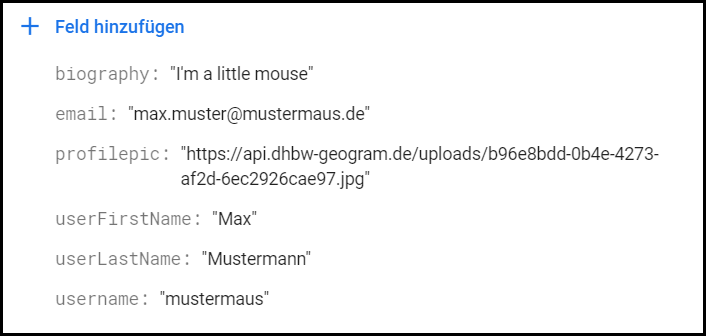
\includegraphics[width=.7\linewidth]{images/collection_users.png}
    \caption{Felder eines \glqq users\grqq{}-Dokumentes}
    \label{fig:users_collection}
\end{figure}

Die Dokumente der Sammlung \glqq images\grqq{} bilden die verschiedenen Bilder von Geogram ab. Ein Bild wird durch folgende Felder definiert:

\begin{itemize}
    \item \textbf{comments}: Array mit allen Kommentaren und dazugehörigen Informationen
    \item \textbf{description}: Beschreibung des Bildes
    \item \textbf{id}: Eindeutige Id für das Bild
    \item \textbf{location}: GPS-Informationen für das Bild
    \item \textbf{timestamp}: Zeitpunkt des Hochladens des Bildes
    \item \textbf{title}: Titel des Bildes
    \item \textbf{url}: URL zu dem Bild, welches im Foto-Server abgespeichert ist
    \item \textbf{user}: Username des Bild-Inhabers
\end{itemize}

In \autoref{fig:images_collection} ist ein beispielhaftes images-Dokument abgebildet.

\begin{figure}[H]
    \centering
    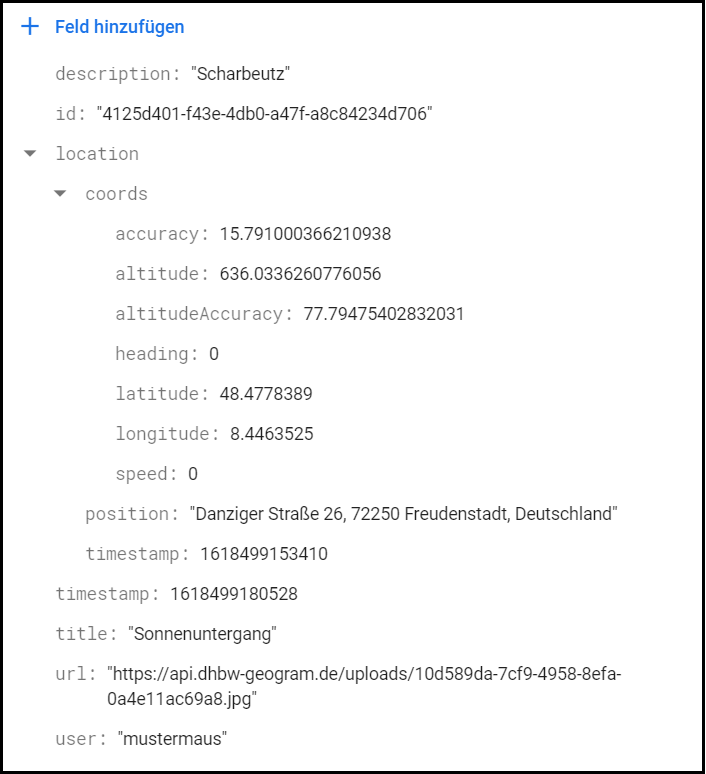
\includegraphics[width=.7\linewidth]{images/collection_images.png}
    \caption{Felder eines \glqq images\grqq{}-Dokumentes}
    \label{fig:images_collection}
\end{figure}

\subsection{Foto-Server\label{sup3.2.3:Unterpunkt-3}}

Um das kostenpflichtige Lizenzmodell von Firebase zu umgehen, wurde ein eigener Foto-Server bereitsgestellt. Aufgrund des begrenzten Speicherplatzes (max. 1 GiB) im Firestore, werden nur noch die URL-Adressen der jeweiligen Bilder im Firestore abgelegt. Zu sehen ist das Abspeichern der URL-Adressen in den Abbildungen \autoref{fig:users_collection} und \autoref{fig:images_collection}. Die URL-Adressen sind alle nach folgendem URL-Schema aufgebaut:

\noindent\fbox{%
    \parbox{\textwidth}{%
        \url{https://api.dhbw-geogram.de/uploads/{image_id}.jpg}
    }%
}

Für die Umsetzung des Foto-Servers wurde sich für das Web-Framework \glqq Express\grqq{} entschieden. Es zählt zu den bekanntesten Web-Frameworks, welche in der Node.js Laufzeitumgebung beheimatet ist.

Für die Verarbeitung von eingehenden Web-Anfragen, verwendet Express eine Art Pipeline-Mechanismus. In \autoref{lst:expressFotoServer} ist ein Ausschnitt aus dem Quellcode des Foto-Servers abgebildet. Im Code wird hierfür zunächst ein Express-Objekt erstellt. Mit der use-Methode können der Pipeline verschiedene Middlewares hinzugefügt werden. So gibt es zum Beispiel die Möglichkeit, bei der Verarbeitung der Web-Anfrage, einen Logger oder JSON-Parser hinzuzufügen. Die Express-Pipeline orientiert sich am REST-Paradigma. Der Foto-Server hat daher die get- und post-Methoden implementiert. Mit den beiden Methoden besteht die Möglichkeit ein Foto entweder dem Server hinzuzufügen (post) oder abzufragen (get).

\begin{lstlisting}[label=lst:expressFotoServer, caption={Codeausschnitt aus dem Foto-Server}, captionpos=b]
    ...

    var app = express();

    app.use(logger("dev"));
    app.use(express.json({ limit: "50mb" }));
    app.use(express.urlencoded({ extended: false, limit: "50mb" }));
    app.use(cookieParser());
    app.use(express.static(path.join(__dirname, "public")));
    app.use(cors());

    app.get("/upload1/:data", (req, res) => {
        ...
    )};

    app.post("/upload1", (req, res) => {
        ...
    )};

    ...
\end{lstlisting}

Gehostet und verwaltet wird der Foto-Server, wie beschrieben, von Paul Finkbeiner. 